\documentclass[12pt,a4paper]{article}

% ─── Page Layout ───────────────────────────────────────────────────────────────
\usepackage[a4paper, margin=0.8in, headheight=14pt]{geometry}

% ─── Fonts (XeLaTeX) ───────────────────────────────────────────────────────────
\usepackage{fontspec}
\usepackage{unicode-math}
\setmainfont{TeX Gyre Pagella}
\setmonofont[Scale=0.88]{TeX Gyre Cursor}
\setmathfont{Latin Modern Math}

% ─── Packages ──────────────────────────────────────────────────────────────────
\usepackage{xcolor}
\usepackage{colortbl}
\usepackage{titlesec}
\usepackage{enumitem}
\usepackage{tabularx}
\usepackage{booktabs}
\usepackage{array}
\usepackage{amsmath}
\usepackage{tikz}
\usetikzlibrary{shapes.geometric, arrows.meta, positioning, calc, fit, decorations.pathreplacing, patterns}
\usepackage{tcolorbox}
\tcbuselibrary{skins, breakable}
\usepackage{hyperref}
\usepackage{fancyhdr}
\usepackage{graphicx}
\usepackage{microtype}
\hyphenpenalty=10000
\exhyphenpenalty=10000
\sloppy
\usepackage{caption}
\usepackage{setspace}
\usepackage{multirow}
\usepackage{tocloft}

% ─── Q&A helper ────────────────────────────────────────────────────────────────
\newcommand{\Q}[1]{\textbf{#1}\par\noindent\ignorespaces}

% ─── Colour Palette ────────────────────────────────────────────────────────────
\definecolor{myred}{RGB}{196,30,58}
\definecolor{mydark}{RGB}{30,30,50}
\definecolor{mygreen}{RGB}{14,120,80}
\definecolor{myteal}{RGB}{0,130,140}
\definecolor{myamber}{RGB}{180,100,0}
\definecolor{mypurple}{RGB}{100,30,160}
\definecolor{mygray}{RGB}{246,247,249}
\definecolor{mgframe}{RGB}{180,185,200}
\definecolor{watermark}{RGB}{145,150,170}
\definecolor{hdrred}{RGB}{250,232,235}
\definecolor{hdrgreen}{RGB}{220,244,233}
\definecolor{hdrteal}{RGB}{220,242,244}
\definecolor{hdramber}{RGB}{253,242,215}
\definecolor{hdrpurple}{RGB}{238,228,255}
\definecolor{hdrgray}{RGB}{238,240,245}
\definecolor{rowalt}{RGB}{250,251,253}

% ─── Section Formatting ────────────────────────────────────────────────────────
\titleformat{\section}
  {\large\bfseries\color{myred}}{\thesection.}{0.5em}{}
  [\vspace{1pt}{\color{myred}\rule{\linewidth}{0.8pt}}]
\titleformat{\subsection}
  {\normalsize\bfseries\color{myteal}}{\thesubsection}{0.5em}{}
\titlespacing*{\section}{0pt}{18pt}{7pt}
\titlespacing*{\subsection}{0pt}{11pt}{4pt}

% ─── Paragraph ─────────────────────────────────────────────────────────────────
\setlength{\parindent}{0pt}
\setlength{\parskip}{4pt}

% ─── TOC Styling ───────────────────────────────────────────────────────────────
\renewcommand{\cfttoctitlefont}{\large\bfseries\color{myred}}
\renewcommand{\cftaftertoctitle}{\par\noindent{\color{myred}\rule{\linewidth}{0.8pt}}}
\setlength{\cftbeforetoctitleskip}{0pt}
\setlength{\cftaftertoctitleskip}{6pt}
\renewcommand{\cftsecfont}{\normalsize\bfseries\color{mydark}}
\renewcommand{\cftsecpagefont}{\normalsize\bfseries\color{mydark}}
\renewcommand{\cftsecleader}{\cftdotfill{\cftdotsep}}
\setlength{\cftbeforesecskip}{7pt}
\renewcommand{\cftsubsecfont}{\small\color{mydark}}
\renewcommand{\cftsubsecpagefont}{\small\color{mydark}}
\setlength{\cftbeforesubsecskip}{3pt}
\setlength{\cftsubsecindent}{1.4em}

% ─── Table helpers ─────────────────────────────────────────────────────────────
\renewcommand{\arraystretch}{1.45}
\setlength{\tabcolsep}{6pt}
\arrayrulecolor{mydark}
\newcolumntype{B}[1]{>{\small\bfseries\raggedright\arraybackslash}m{#1}}
\newcolumntype{Y}{>{\small\raggedright\arraybackslash}X}
\renewcommand{\tabularxcolumn}[1]{m{#1}}

% ─── Header / Footer ───────────────────────────────────────────────────────────
\pagestyle{fancy}
\fancyhf{}
\fancyhead[L]{\small\color{myred}\textbf{EC302}\;\color{mydark}--- Digital System Design}
\fancyhead[R]{\small\color{myteal}\textbf{Module 4 Notes}}
\fancyfoot[C]{\small\color{mydark}\thepage}
\fancyfoot[R]{\small\color{watermark}\textit{\copyright\ Biraj}}
\renewcommand{\headrulewidth}{0.5pt}
\renewcommand{\footrulewidth}{0.3pt}

% ─── Hyperref ──────────────────────────────────────────────────────────────────
\hypersetup{
  colorlinks=true, linkcolor=myteal, urlcolor=myteal,
  pdfauthor={Biraj Sarkar (CGEC)},
  pdftitle={EC302 --- Module 4 Notes: VLSI Design Flow and VHDL Modeling}
}

% ─── tcolorbox styles ──────────────────────────────────────────────────────────
\tcbset{
  tikzbox/.style={
    colback=mygray, colframe=mgframe, boxrule=0.6pt, arc=4pt,
    left=8pt, right=8pt, top=6pt, bottom=6pt,
    colbacktitle=mgframe, coltitle=mydark,
    fonttitle=\small\bfseries
  },
  defbox/.style={
    colback=hdrgreen, colframe=mygreen, boxrule=0.8pt, arc=4pt,
    left=9pt, right=9pt, top=6pt, bottom=6pt,
    colbacktitle=mygreen, coltitle=white,
    fonttitle=\small\bfseries
  },
  formulabox/.style={
    colback=hdrteal, colframe=myteal, boxrule=0.8pt, arc=4pt,
    left=9pt, right=9pt, top=6pt, bottom=6pt,
    colbacktitle=myteal, coltitle=white,
    fonttitle=\small\bfseries
  },
  examplebox/.style={
    colback=hdramber, colframe=myamber, boxrule=0.8pt, arc=4pt,
    left=9pt, right=9pt, top=6pt, bottom=6pt,
    colbacktitle=myamber, coltitle=white,
    fonttitle=\small\bfseries
  },
  masonbox/.style={
    colback=hdrpurple, colframe=mypurple, boxrule=0.8pt, arc=4pt,
    left=9pt, right=9pt, top=6pt, bottom=6pt,
    colbacktitle=mypurple, coltitle=white,
    fonttitle=\small\bfseries
  },
  exambox/.style={
    colback=hdrpurple, colframe=mypurple, boxrule=1pt, arc=5pt,
    left=10pt, right=10pt, top=8pt, bottom=8pt,
    colbacktitle=mypurple, coltitle=white,
    fonttitle=\bfseries,
    breakable, title after break={\textbf{Frequently Asked / Viva Questions (contd.)}}
  }
}

\tcbset{breakable}
\tcbset{after={\color{black}}}

% ─── TikZ styles ───────────────────────────────────────────────────────────────
\tikzset{
  vlsiblock/.style={rectangle, draw=myteal, fill=hdrteal,
    minimum width=2.4cm, minimum height=1.1cm,
    font=\small\bfseries, rounded corners=3pt, line width=0.8pt, align=center},
  flowarrow/.style={-Stealth, thick, color=mydark}
}

\begin{document}

% ─── Title Page ───────────────────────────────────────────────────────────────
\begin{center}
  {\LARGE\bfseries\color{myred} EC302 --- Digital System Design}\\[5pt]
  {\normalsize\color{mydark} Semester III \quad$\bullet$\quad 3L:0T:0P \quad$\bullet$\quad 3 Credits}\\[3pt]
  {\normalsize\color{myteal}\textbf{Module 4 Exam Notes: VLSI Design Flow \& VHDL Modeling}}\\[3pt]
  {\small\color{mydark} CGEC \;$|$\; B.Tech ECE (2023--27) \;$|$\; \textit{Biraj Sarkar}}
\end{center}
\vspace{2pt}
\noindent{\color{myred}\rule{\linewidth}{1.5pt}}
\vspace{2pt}

\hypersetup{linkcolor=mydark}
\tableofcontents
\hypersetup{linkcolor=myteal}
\newpage

% ===============================================================================
\section{The VLSI Design Flow and Methodologies}
% ===============================================================================

Very Large Scale Integration (VLSI) design is the systematic transformation of an abstract architectural system specification into a physically verified, fabricated silicon integrated circuit containing millions to billions of transistors.

\subsection{The Gajski-Kuhn Y-Chart}
The Gajski-Kuhn Y-chart visualizes VLSI design complexity across three distinct \textbf{domains of representation} intersecting at concentric \textbf{levels of abstraction}:
\begin{itemize}[leftmargin=*, itemsep=3pt]
  \item \textbf{Behavioral Domain (What it does):} Specifies functional algorithms, equations, input-output relationships, and state transitions without detailing physical hardware.
  \item \textbf{Structural Domain (How it is composed):} Defines hardware entities as interconnections of structural sub-blocks, modules, logic gates, and transistors.
  \item \textbf{Physical / Geometric Domain (How it is built):} Represents physical implementation as silicon geometric masks, transistor layouts, placement coordinates, and metallization routing tracks.
  \item \textbf{Levels of Abstraction:} Architectural / System level $\to$ Algorithmic level $\to$ Register-Transfer Level (RTL) $\to$ Logic / Gate level $\to$ Transistor / Circuit level $\to$ Mask layout level.
\end{itemize}

\subsection{Step-by-Step Modern Digital ASIC and FPGA Design Flow}
\begin{enumerate}[label=\arabic*., leftmargin=*]
  \item \textbf{System Specification \& Architecture Planning:} Defines system throughput, clock frequency, word width, power budget, and interface protocols.
  \item \textbf{Design Entry:} Entering the digital design into CAD tools:
    \begin{itemize}
      \item \textit{Schematic Capture:} Graphical drawing of interconnected logic gates. Intuitive for small designs; unmanageable for complex million-gate chips.
      \item \textit{State Diagram / FSM Entry:} Graphical specification of states, transitions, and outputs; automatically compiled into HDL code.
      \item \textit{Hardware Description Languages (HDLs):} Textual algorithmic descriptions using VHDL, Verilog, or SystemVerilog. Standard for modern complex VLSI.
    \end{itemize}
  \item \textbf{Functional (RTL) Simulation:} Verifies behavioral and logic correctness using an HDL testbench. Assumes ideal zero-delay or unit-delay gates to detect algorithmic bugs early.
  \item \textbf{Logic Synthesis:} CAD tool (e.g., Synopsys Design Compiler, Vivado) translates abstract RTL code into an optimized, technology-specific \textbf{gate-level netlist} mapped to standard cells (AND, NAND, Flip-Flops) from a target semiconductor library, driven by designer constraints (target clock period, maximum silicon area, dynamic power).
  \item \textbf{Gate-Level Netlist Simulation:} Simulates the synthesized gate netlist to confirm that synthesis introduced no unintended logic changes or state mismatches.
  \item \textbf{Static Timing Analysis (STA):} Exhaustively evaluates path delays to guarantee that clock setup and hold time requirements are met for every register without dynamic vectors:
    \begin{align}
      \text{Setup Time Constraint:} \quad & T_{\text{clk}} \ge t_{cq} + t_{\text{comb}(\max)} + t_{\text{setup}} - t_{\text{skew}} \\
      \text{Hold Time Constraint:} \quad & t_{cq} + t_{\text{comb}(\min)} \ge t_{\text{hold}} + t_{\text{skew}}
    \end{align}
  \item \textbf{Physical Design (P\&R - Place and Route):}
    \begin{itemize}
      \item \textit{Floorplanning:} Allocates chip area for major functional blocks, I/O pads, and power/ground grids ($V_{DD}, V_{SS}$).
      \item \textit{Placement:} Determines exact $(x, y)$ coordinate locations for every standard cell.
      \item \textit{Clock Tree Synthesis (CTS):} Constructs balanced clock distribution networks (H-tree) to minimize clock skew ($t_{\text{skew}}$) and insertion delay.
      \item \textit{Routing:} Wires together all cell pins using multi-layer metallization.
    \end{itemize}
  \item \textbf{Parasitic Extraction and Post-Layout Timing Verification:} Extracts parasitic resistances ($R$) and capacitances ($C$) from actual layout geometries and back-annotates them into a Standard Delay Format (SDF) file for final timing sign-off.
  \item \textbf{Physical Verification:}
    \begin{itemize}
      \item \textit{DRC (Design Rule Checking):} Verifies that geometric shapes satisfy foundry manufacturing rules (minimum metal width, spacing, enclosure).
      \item \textit{LVS (Layout Versus Schematic):} Extracts electrical transistor circuits from the physical layout and compares connectivity netlists 1-to-1 against the schematic.
    \end{itemize}
  \item \textbf{Tape-out:} Exporting final layout data in GDSII / OASIS stream format to the semiconductor foundry for photolithographic mask fabrication (or generating a configuration bitstream for an FPGA).
\end{enumerate}

\begin{tcolorbox}[tikzbox, title={Digital VLSI / ASIC Design Flow Pipeline}]
\centering
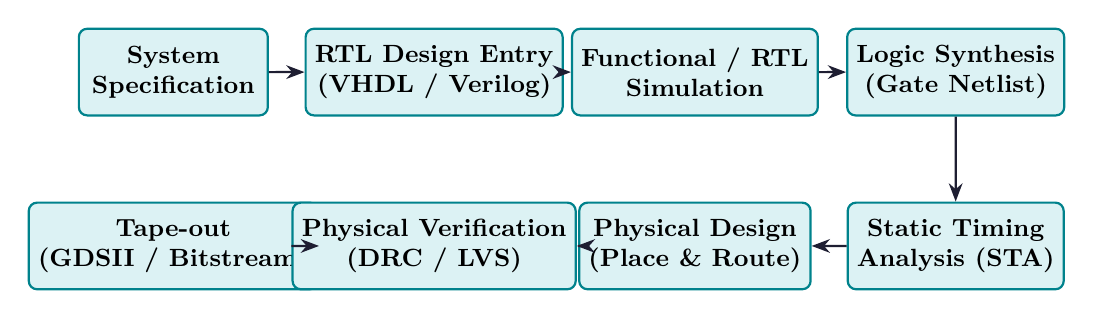
\begin{tikzpicture}[scale=0.92]
  \node[vlsiblock] (s1) at (0, 3.6) {System\\Specification};
  \node[vlsiblock] (s2) at (3.6, 3.6) {RTL Design Entry\\(VHDL / Verilog)};
  \node[vlsiblock] (s3) at (7.2, 3.6) {Functional / RTL\\Simulation};
  \node[vlsiblock] (s4) at (10.8, 3.6) {Logic Synthesis\\(Gate Netlist)};

  \node[vlsiblock] (s8) at (0, 1.2) {Tape-out\\(GDSII / Bitstream)};
  \node[vlsiblock] (s7) at (3.6, 1.2) {Physical Verification\\(DRC / LVS)};
  \node[vlsiblock] (s6) at (7.2, 1.2) {Physical Design\\(Place \& Route)};
  \node[vlsiblock] (s5) at (10.8, 1.2) {Static Timing\\Analysis (STA)};

  \draw[flowarrow] (s1) -- (s2);
  \draw[flowarrow] (s2) -- (s3);
  \draw[flowarrow] (s3) -- (s4);
  \draw[flowarrow] (s4) -- (s5);
  \draw[flowarrow] (s5) -- (s6);
  \draw[flowarrow] (s6) -- (s7);
  \draw[flowarrow] (s7) -- (s8);
\end{tikzpicture}
\end{tcolorbox}

% ===============================================================================
\section{VHDL Language Fundamentals and Structural Units}
% ===============================================================================

VHDL (VHSIC Hardware Description Language) is an IEEE standard (IEEE Std 1076) language designed to model the behavior, dataflow, and structural composition of digital electronic systems across multiple levels of abstraction.

\subsection{Fundamental Design Units of VHDL}
A complete VHDL design entity is composed of primary design units:
\begin{enumerate}[label=\arabic*., leftmargin=*]
  \item \textbf{Library and Package Declarations:} Grants access to pre-compiled packages containing standardized data types, constants, and operators:
\begin{spacing}{1.0}
\begin{verbatim}
LIBRARY IEEE;
USE IEEE.STD_LOGIC_1164.ALL;    -- Imports STD_LOGIC, STD_LOGIC_VECTOR
USE IEEE.NUMERIC_STD.ALL;       -- Imports SIGNED, UNSIGNED arithmetic
\end{verbatim}
\end{spacing}
  \item \textbf{Entity Declaration:} Defines the external hardware boundary and interface ports of the module (the "black box" view):
\begin{spacing}{1.0}
\begin{verbatim}
ENTITY entity_name IS
  GENERIC ( param_name : type := default_val ); -- Optional parameterized constants
  PORT (
    port_name : mode data_type;
    ...
  );
END entity_name;
\end{verbatim}
\end{spacing}
  \item \textbf{Architecture Body:} Defines the internal behavior, logic equations, or structural interconnection of components (the "inside" of the box). Multiple architectures can be written for a single entity (e.g., behavioral vs. structural):
\begin{spacing}{1.0}
\begin{verbatim}
ARCHITECTURE arch_name OF entity_name IS
  -- Declarative region: signals, constants, components, types
BEGIN
  -- Concurrent statements region: processes, component instantiations
END arch_name;
\end{verbatim}
\end{spacing}
  \item \textbf{Configuration Declaration:} Binds specific architecture bodies and component implementations to entity instances in hierarchical designs.
\end{enumerate}

\subsection{VHDL Port Modes}
\par\vspace{6pt}\noindent
\begingroup
\setlength{\tabcolsep}{3.5pt}
\setlength{\extrarowheight}{3pt}
\begin{tabularx}{\linewidth}{|B{2.2cm}|B{3.2cm}|Y|}
\hline
\textbf{Port Mode} & \textbf{Directionality} & \textbf{Internal Architecture Usage} \\
\hline
\texttt{IN} & Input to module & Read-only inside architecture. Cannot be assigned or driven. \\
\hline
\texttt{OUT} & Output from module & Write-only. Values can be assigned to it, but cannot be read internally. \\
\hline
\texttt{INOUT} & Bidirectional & Can be driven and read internally. Requires tri-state resolution. \\
\hline
\texttt{BUFFER} & Output with internal feedback & Drives output pin and allows internal readback. Has restrictive binding rules. \\
\hline
\end{tabularx}
\endgroup

% ===============================================================================
\section{Data Types, Data Objects, and Operators}
% ===============================================================================

\subsection{Data Objects in VHDL}
VHDL supports four classes of data objects:
\begin{itemize}[leftmargin=*, itemsep=4pt]
  \item \textbf{SIGNAL:} Represents physical interconnecting electrical wires or traces.
    \begin{itemize}
      \item Declared in architecture declarative regions or packages; visible throughout the entire architecture.
      \item Updated concurrently with a scheduled propagation delay (delta delay $\delta$).
      \item Assignment operator: \texttt{<=} (e.g., \texttt{Y <= A AND B;}).
    \end{itemize}
  \item \textbf{VARIABLE:} Represents local computational scratchpad storage.
    \begin{itemize}
      \item Declared strictly inside a \texttt{PROCESS}, \texttt{FUNCTION}, or \texttt{PROCEDURE}. Not visible outside.
      \item Updated \textbf{instantaneously} without delay.
      \item Assignment operator: \texttt{:=} (e.g., \texttt{v\_count := v\_count + 1;}).
    \end{itemize}
  \item \textbf{CONSTANT:} Holds a permanent, unmodifiable value established during elaboration. Assignment operator: \texttt{:=} (e.g., \texttt{CONSTANT WIDTH : INTEGER := 8;}).
  \item \textbf{FILE:} Represents external host system files used for automated testbench verification and stimulus vectors.
\end{itemize}

\par\vspace{6pt}\noindent
\begingroup
\setlength{\tabcolsep}{3.5pt}
\setlength{\extrarowheight}{3pt}
\begin{tabularx}{\linewidth}{|B{2.8cm}|Y|Y|}
\hline
\textbf{Property} & \textbf{SIGNAL} & \textbf{VARIABLE} \\
\hline
Hardware Meaning & Physical electrical wire / bus & Local memory / register variable \\
\hline
Declaration Scope & Architecture, package, block & Exclusively inside \texttt{PROCESS} or subprograms \\
\hline
Assignment Operator & \texttt{<=} (Non-blocking, scheduled) & \texttt{:=} (Blocking, instantaneous) \\
\hline
Update Timing & Updated at end of current simulation cycle & Updated immediately when evaluated \\
\hline
Synthesized Hardware & Interconnecting wires, latches, or flip-flops & Internal combinational nodes or registers \\
\hline
\end{tabularx}
\endgroup

\subsection{Standard and IEEE 1164 Data Types}
\begin{itemize}[leftmargin=*, itemsep=3pt]
  \item \textbf{Standard Types:} \texttt{BIT} (\texttt{'0'}, \texttt{'1'}), \texttt{BOOLEAN} (\texttt{TRUE}, \texttt{FALSE}), \texttt{INTEGER} (32-bit minimum range: $-2^{31}$ to $2^{31}-1$), \texttt{CHARACTER}, \texttt{TIME} (e.g., \texttt{10 ns}).
  \item \textbf{IEEE Standard 1164 Multi-Valued Logic (\texttt{STD\_LOGIC}):} Provides realistic modeling of electrical logic states across integrated circuit nodes:
\end{itemize}

\par\vspace{6pt}\noindent
\begingroup
\setlength{\tabcolsep}{3.5pt}
\setlength{\extrarowheight}{3pt}
\begin{tabularx}{\linewidth}{|B{1.6cm}|B{3.2cm}|Y|}
\hline
\textbf{Value} & \textbf{Electrical Meaning} & \textbf{Hardware Significance} \\
\hline
\texttt{'U'} & Uninitialized & Default initial simulation state of unassigned signals \\
\hline
\texttt{'X'} & Forcing Unknown & Unresolvable contention / unknown logic conflict \\
\hline
\texttt{'0'} & Forcing 0 & Strong logic LOW tied to ground ($V_{SS}$) \\
\hline
\texttt{'1'} & Forcing 1 & Strong logic HIGH tied to supply ($V_{DD}$) \\
\hline
\texttt{'Z'} & High Impedance & Tri-state output; electrically disconnected \\
\hline
\texttt{'W'} & Weak Unknown & Weak signal contention \\
\hline
\texttt{'L'} & Weak 0 & Pull-down resistor to ground \\
\hline
\texttt{'H'} & Weak 1 & Pull-up resistor to supply \\
\hline
\texttt{'-'} & Don't Care & Wildcard used in synthesis minimization \\
\hline
\end{tabularx}
\endgroup

\subsection{VHDL Operators}
\begin{itemize}[leftmargin=*, itemsep=2pt]
  \item \textbf{Logical Operators:} \texttt{AND}, \texttt{OR}, \texttt{NAND}, \texttt{NOR}, \texttt{XOR}, \texttt{XNOR}, \texttt{NOT}.
  \item \textbf{Relational Operators:} \texttt{=} (equal), \texttt{/=} (not equal), \texttt{<}, \texttt{<=}, \texttt{>}, \texttt{>=}.
  \item \textbf{Arithmetic Operators:} \texttt{+} (addition), \texttt{-} (subtraction), \texttt{*} (multiplication), \texttt{/} (division), \texttt{MOD}, \texttt{REM}, \texttt{ABS}, \texttt{**} (exponentiation).
  \item \textbf{Concatenation Operator (\texttt{\&}):} Combines scalars or vectors into wider vectors (e.g., \texttt{Y <= A \& B;}).
\end{itemize}

% ===============================================================================
\section{VHDL Modeling Styles and Coding Methodologies}
% ===============================================================================

Digital hardware architectures can be expressed using three distinct modeling styles:

\subsection{Dataflow (Concurrent) Modeling}
Expresses hardware as continuous concurrent signal assignments that execute simultaneously whenever any right-hand-side operand changes:
\begin{itemize}[leftmargin=*, itemsep=3pt]
  \item \textbf{Simple Concurrent Assignment:} \texttt{Y <= A AND B;}
  \item \textbf{Conditional Signal Assignment (\texttt{WHEN-ELSE}):}
\begin{spacing}{1.0}
\begin{verbatim}
Y <= A WHEN (Sel = "00") ELSE
     B WHEN (Sel = "01") ELSE
     C WHEN (Sel = "10") ELSE D;
\end{verbatim}
\end{spacing}
  \item \textbf{Selected Signal Assignment (\texttt{WITH-SELECT}):}
\begin{spacing}{1.0}
\begin{verbatim}
WITH Sel SELECT
  Y <= A WHEN "00",
       B WHEN "01",
       C WHEN "10",
       D WHEN OTHERS;
\end{verbatim}
\end{spacing}
\end{itemize}

\subsection{Behavioral (Sequential) Modeling}
Specifies the algorithmic behavior of the hardware within a \textbf{\texttt{PROCESS}} block. Statements inside a process execute sequentially from top to bottom, but the process block itself is evaluated concurrently relative to the rest of the architecture:
\begin{itemize}[leftmargin=*, itemsep=3pt]
  \item \textbf{Sensitivity List:} A list of signals enclosed in parentheses following the \texttt{PROCESS} keyword. The process activates whenever any signal in its sensitivity list transitions:
\begin{spacing}{1.0}
\begin{verbatim}
PROCESS (clk, reset) -- Activated on transitions of clk or reset
BEGIN
  IF (reset = '1') THEN
    Q <= '0';
  ELSIF rising_edge(clk) THEN
    Q <= D;
  END IF;
END PROCESS;
\end{verbatim}
\end{spacing}
  \item \textbf{Sequential Control Statements:} \texttt{IF-THEN-ELSIF-ELSE}, \texttt{CASE-WHEN}, \texttt{FOR-LOOP}, \texttt{WHILE-LOOP}.
\end{itemize}

\begin{tcolorbox}[defbox, title={\textbf{Critical Synthesis Hazard: Inferred Latches}}]
In combinational processes, if an \texttt{IF} statement lacks a complete \texttt{ELSE} clause, or a \texttt{CASE} statement omits the \texttt{WHEN OTHERS} branch or fails to assign every output signal across all possible input permutations, the synthesis tool must infer a \textbf{transparent latch} to preserve the previous output state. This creates asynchronous hazards, degrades timing closure, and must be prevented by assigning unambiguous default values at the top of every combinational process.
\end{tcolorbox}

\subsection{Structural Modeling}
Describes a system hierarchically by declaring pre-designed sub-components and mapping their ports together like an electrical schematic:
\begin{enumerate}[label=\arabic*., leftmargin=*]
  \item Declare component interface in architecture declarative region.
  \item Instantiate components in architecture body and connect signals using \texttt{PORT MAP}.
\end{enumerate}

% ===============================================================================
\section{VHDL Code Library for Combinational Logic Circuits}
% ===============================================================================

\begin{tcolorbox}[examplebox, title={1. Half Adder and Full Adder (Dataflow, Behavioral, Structural)}]
\begin{spacing}{0.95}
\begin{verbatim}
-- Half Adder (Dataflow)
LIBRARY IEEE;
USE IEEE.STD_LOGIC_1164.ALL;
ENTITY half_adder IS
  PORT ( A, B : IN STD_LOGIC; Sum, Cout : OUT STD_LOGIC );
END half_adder;
ARCHITECTURE dataflow OF half_adder IS
BEGIN
  Sum  <= A XOR B;
  Cout <= A AND B;
END dataflow;

-- Full Adder (Structural using 2 Half Adders + OR Gate)
LIBRARY IEEE;
USE IEEE.STD_LOGIC_1164.ALL;
ENTITY full_adder IS
  PORT ( A, B, Cin : IN STD_LOGIC; Sum, Cout : OUT STD_LOGIC );
END full_adder;
ARCHITECTURE structural OF full_adder IS
  COMPONENT half_adder
    PORT ( A, B : IN STD_LOGIC; Sum, Cout : OUT STD_LOGIC );
  END COMPONENT;
  SIGNAL s1, c1, c2 : STD_LOGIC;
BEGIN
  HA1: half_adder PORT MAP ( A => A, B => B, Sum => s1, Cout => c1 );
  HA2: half_adder PORT MAP ( A => s1, B => Cin, Sum => Sum, Cout => c2 );
  Cout <= c1 OR c2;
END structural;
\end{verbatim}
\end{spacing}
\end{tcolorbox}

\begin{tcolorbox}[examplebox, title={2. 4-to-1 Multiplexer (Dataflow and Behavioral)}]
\begin{spacing}{0.95}
\begin{verbatim}
LIBRARY IEEE;
USE IEEE.STD_LOGIC_1164.ALL;

ENTITY mux4to1 IS
  PORT (
    D   : IN  STD_LOGIC_VECTOR(3 DOWNTO 0);
    Sel : IN  STD_LOGIC_VECTOR(1 DOWNTO 0);
    Y   : OUT STD_LOGIC
  );
END mux4to1;

ARCHITECTURE behavioral OF mux4to1 IS
BEGIN
  PROCESS (D, Sel)
  BEGIN
    CASE Sel IS
      WHEN "00" => Y <= D(0);
      WHEN "01" => Y <= D(1);
      WHEN "10" => Y <= D(2);
      WHEN "11" => Y <= D(3);
      WHEN OTHERS => Y <= '0';
    END CASE;
  END PROCESS;
END behavioral;
\end{verbatim}
\end{spacing}
\end{tcolorbox}

\begin{tcolorbox}[examplebox, title={3. 2-to-4 Binary Decoder with Active-Low Enable}]
\begin{spacing}{0.95}
\begin{verbatim}
LIBRARY IEEE;
USE IEEE.STD_LOGIC_1164.ALL;

ENTITY decoder2to4 IS
  PORT (
    A     : IN  STD_LOGIC_VECTOR(1 DOWNTO 0);
    En_n  : IN  STD_LOGIC;                     -- Active-low enable
    Y     : OUT STD_LOGIC_VECTOR(3 DOWNTO 0)   -- Active-high outputs
  );
END decoder2to4;

ARCHITECTURE dataflow OF decoder2to4 IS
BEGIN
  Y <= "0001" WHEN (En_n = '0' AND A = "00") ELSE
       "0010" WHEN (En_n = '0' AND A = "01") ELSE
       "0100" WHEN (En_n = '0' AND A = "10") ELSE
       "1000" WHEN (En_n = '0' AND A = "11") ELSE
       "0000";
END dataflow;
\end{verbatim}
\end{spacing}
\end{tcolorbox}

\begin{tcolorbox}[examplebox, title={4. 4-Bit Arithmetic Logic Unit (ALU)}]
\begin{spacing}{0.95}
\begin{verbatim}
LIBRARY IEEE;
USE IEEE.STD_LOGIC_1164.ALL;
USE IEEE.NUMERIC_STD.ALL;

ENTITY alu_4bit IS
  PORT (
    A, B   : IN  STD_LOGIC_VECTOR(3 DOWNTO 0);
    Op     : IN  STD_LOGIC_VECTOR(2 DOWNTO 0);
    Result : OUT STD_LOGIC_VECTOR(3 DOWNTO 0);
    Cout   : OUT STD_LOGIC
  );
END alu_4bit;

ARCHITECTURE behavioral OF alu_4bit IS
BEGIN
  PROCESS (A, B, Op)
    VARIABLE temp : UNSIGNED(4 DOWNTO 0);
  BEGIN
    Cout <= '0';
    CASE Op IS
      WHEN "000" => -- ADD
        temp := ('0' & UNSIGNED(A)) + ('0' & UNSIGNED(B));
        Result <= STD_LOGIC_VECTOR(temp(3 DOWNTO 0));
        Cout   <= temp(4);
      WHEN "001" => -- SUBTRACT
        temp := ('0' & UNSIGNED(A)) - ('0' & UNSIGNED(B));
        Result <= STD_LOGIC_VECTOR(temp(3 DOWNTO 0));
      WHEN "010" => -- AND
        Result <= A AND B;
      WHEN "011" => -- OR
        Result <= A OR B;
      WHEN "100" => -- XOR
        Result <= A XOR B;
      WHEN "101" => -- NOT A
        Result <= NOT A;
      WHEN OTHERS =>
        Result <= "0000";
    END CASE;
  END PROCESS;
END behavioral;
\end{verbatim}
\end{spacing}
\end{tcolorbox}

% ===============================================================================
\section{VHDL Code Library for Sequential Logic Circuits}
% ===============================================================================

\begin{tcolorbox}[examplebox, title={1. D Flip-Flop with Asynchronous Active-Low Reset}]
\begin{spacing}{0.95}
\begin{verbatim}
LIBRARY IEEE;
USE IEEE.STD_LOGIC_1164.ALL;

ENTITY d_flip_flop IS
  PORT (
    clk     : IN  STD_LOGIC;
    rst_n   : IN  STD_LOGIC; -- Asynchronous active-low reset
    d       : IN  STD_LOGIC;
    q, q_bar: OUT STD_LOGIC
  );
END d_flip_flop;

ARCHITECTURE behavioral OF d_flip_flop IS
  SIGNAL q_reg : STD_LOGIC;
BEGIN
  PROCESS (clk, rst_n)
  BEGIN
    IF (rst_n = '0') THEN
      q_reg <= '0';
    ELSIF rising_edge(clk) THEN
      q_reg <= d;
    END IF;
  END PROCESS;
  q     <= q_reg;
  q_bar <= NOT q_reg;
END behavioral;
\end{verbatim}
\end{spacing}
\end{tcolorbox}

\begin{tcolorbox}[examplebox, title={2. 4-Bit Synchronous Up-Counter with Parallel Load}]
\begin{spacing}{0.95}
\begin{verbatim}
LIBRARY IEEE;
USE IEEE.STD_LOGIC_1164.ALL;
USE IEEE.NUMERIC_STD.ALL;

ENTITY counter_4bit IS
  PORT (
    clk    : IN  STD_LOGIC;
    rst_n  : IN  STD_LOGIC;                     -- Asynchronous active-low reset
    load   : IN  STD_LOGIC;                     -- Synchronous load enable
    en     : IN  STD_LOGIC;                     -- Count enable
    d_in   : IN  STD_LOGIC_VECTOR(3 DOWNTO 0);
    q_out  : OUT STD_LOGIC_VECTOR(3 DOWNTO 0)
  );
END counter_4bit;

ARCHITECTURE behavioral OF counter_4bit IS
  SIGNAL count : UNSIGNED(3 DOWNTO 0);
BEGIN
  PROCESS (clk, rst_n)
  BEGIN
    IF (rst_n = '0') THEN
      count <= (OTHERS => '0');
    ELSIF rising_edge(clk) THEN
      IF (load = '1') THEN
        count <= UNSIGNED(d_in);
      ELSIF (en = '1') THEN
        count <= count + 1;
      END IF;
    END IF;
  END PROCESS;
  q_out <= STD_LOGIC_VECTOR(count);
END behavioral;
\end{verbatim}
\end{spacing}
\end{tcolorbox}

\begin{tcolorbox}[examplebox, title={3. 4-Bit Universal Shift Register}]
\begin{spacing}{0.95}
\begin{verbatim}
LIBRARY IEEE;
USE IEEE.STD_LOGIC_1164.ALL;

ENTITY universal_shift_reg IS
  PORT (
    clk    : IN  STD_LOGIC;
    rst_n  : IN  STD_LOGIC;
    mode   : IN  STD_LOGIC_VECTOR(1 DOWNTO 0); -- 00: Hold, 01: Right, 10: Left, 11: Load
    sin_r  : IN  STD_LOGIC;                     -- Serial input for shift-right
    sin_l  : IN  STD_LOGIC;                     -- Serial input for shift-left
    pin    : IN  STD_LOGIC_VECTOR(3 DOWNTO 0);  -- Parallel data in
    pout   : OUT STD_LOGIC_VECTOR(3 DOWNTO 0)   -- Parallel data out
  );
END universal_shift_reg;

ARCHITECTURE behavioral OF universal_shift_reg IS
  SIGNAL r_reg : STD_LOGIC_VECTOR(3 DOWNTO 0);
BEGIN
  PROCESS (clk, rst_n)
  BEGIN
    IF (rst_n = '0') THEN
      r_reg <= (OTHERS => '0');
    ELSIF rising_edge(clk) THEN
      CASE mode IS
        WHEN "00" => r_reg <= r_reg;                   -- Hold
        WHEN "01" => r_reg <= sin_r & r_reg(3 DOWNTO 1); -- Shift Right
        WHEN "10" => r_reg <= r_reg(2 DOWNTO 0) & sin_l; -- Shift Left
        WHEN "11" => r_reg <= pin;                     -- Parallel Load
        WHEN OTHERS => NULL;
      END CASE;
    END IF;
  END PROCESS;
  pout <= r_reg;
END behavioral;
\end{verbatim}
\end{spacing}
\end{tcolorbox}

\begin{tcolorbox}[examplebox, title={4. FSM Sequence Detector for Pattern "1011" (Overlapping Mealy Machine)}]
\begin{spacing}{0.95}
\begin{verbatim}
LIBRARY IEEE;
USE IEEE.STD_LOGIC_1164.ALL;

ENTITY seq_detector_1011 IS
  PORT (
    clk   : IN  STD_LOGIC;
    rst_n : IN  STD_LOGIC;
    din   : IN  STD_LOGIC;
    dout  : OUT STD_LOGIC
  );
END seq_detector_1011;

ARCHITECTURE fsm_arch OF seq_detector_1011 IS
  TYPE state_type IS (S0, S1, S10, S101);
  SIGNAL state_reg, next_state : state_type;
BEGIN
  -- Process 1: State Register (Synchronous)
  PROCESS (clk, rst_n)
  BEGIN
    IF (rst_n = '0') THEN
      state_reg <= S0;
    ELSIF rising_edge(clk) THEN
      state_reg <= next_state;
    END IF;
  END PROCESS;

  -- Process 2: Next State and Output Logic (Combinational)
  PROCESS (state_reg, din)
  BEGIN
    dout <= '0';
    next_state <= state_reg;
    CASE state_reg IS
      WHEN S0 =>
        IF (din = '1') THEN next_state <= S1; ELSE next_state <= S0; END IF;
      WHEN S1 =>
        IF (din = '0') THEN next_state <= S10; ELSE next_state <= S1; END IF;
      WHEN S10 =>
        IF (din = '1') THEN next_state <= S101; ELSE next_state <= S0; END IF;
      WHEN S101 =>
        IF (din = '1') THEN
          dout <= '1'; -- Pattern "1011" detected!
          next_state <= S1; -- Overlapping: prefix "1" retained
        ELSE
          next_state <= S10;
        END IF;
    END CASE;
  END PROCESS;
END fsm_arch;
\end{verbatim}
\end{spacing}
\end{tcolorbox}

\newpage
% ===============================================================================
% MANDATORY QUICK REVISION PAGE
% ===============================================================================
\begin{center}
  {\large\bfseries\color{myred} Quick Revision --- Module 4}\\[3pt]
  {\small\color{mydark} VLSI Design Flow \& VHDL Hardware Modeling $|$ EC302}
\end{center}
\noindent{\color{myred}\rule{\linewidth}{1.2pt}}
\vspace{4pt}

\begin{tcolorbox}[formulabox, title={\textbf{Key Timing Constraints and VHDL Skeletons at a Glance}}]
\renewcommand{\arraystretch}{1.35}
\begin{tabularx}{\linewidth}{B{5.2cm} X}
Setup Time Constraint & $T_{\text{clk}} \ge t_{cq} + t_{\text{comb}(\max)} + t_{\text{setup}} - t_{\text{skew}}$ \\[4pt]
Maximum Clock Frequency & $f_{\max} = \frac{1}{T_{\text{clk}(\min)}}$ \\[4pt]
Hold Time Constraint & $t_{cq} + t_{\text{comb}(\min)} \ge t_{\text{hold}} + t_{\text{skew}} \quad (\text{independent of } T_{\text{clk}})$ \\[4pt]
Dynamic Power Dissipation & $P_{\text{dyn}} = \alpha \cdot C_L \cdot V_{DD}^2 \cdot f$ \\[4pt]
Entity Declaration Skeleton & \texttt{ENTITY name IS PORT (...); END name;} \\[4pt]
Architecture Body Skeleton & \texttt{ARCHITECTURE arch OF name IS ... BEGIN ... END arch;} \\[4pt]
Process Trigger Mechanism & \texttt{PROCESS (clk, reset) BEGIN ... END PROCESS;} \\[4pt]
\end{tabularx}
\end{tcolorbox}

\begin{tcolorbox}[defbox, title={\textbf{One-Line Definitions}}]
\begin{itemize}[leftmargin=*, itemsep=2pt, topsep=0pt]
  \item \textbf{Logic Synthesis:} The automated translation of abstract RTL code into an optimized gate netlist mapped to standard library cells.
  \item \textbf{Static Timing Analysis (STA):} A vector-independent CAD technique verifying setup and hold timing across all paths.
  \item \textbf{Clock Skew:} The difference in clock arrival times at two distinct registers caused by routing differences.
  \item \textbf{VHDL Entity:} The primary design unit defining external hardware interface ports and generic parameters.
  \item \textbf{VHDL Architecture:} The design unit describing internal hardware dataflow, algorithmic behavior, or structural netlist.
  \item \textbf{SIGNAL in VHDL:} A hardware object representing physical interconnecting wires, scheduled with delta delay.
  \item \textbf{VARIABLE in VHDL:} A local computational object evaluated sequentially and updated instantaneously inside a process.
  \item \textbf{Inferred Latch:} An unintended transparent latch generated by synthesis due to incomplete conditional assignments.
  \item \textbf{Sensitivity List:} The list of trigger signals in a process header; the process evaluates when any listed signal changes.
  \item \textbf{DRC (Design Rule Check):} CAD verification ensuring physical layout geometries comply with foundry manufacturing rules.
\end{itemize}
\end{tcolorbox}

\begin{tcolorbox}[exambox, title={\textbf{Frequently Asked / Viva Questions}}]
\begin{enumerate}[topsep=0pt, label=\textbf{Q\arabic*.}, itemsep=5pt]
  \item \Q{What is the difference between a SIGNAL and a VARIABLE in VHDL?}
  A \texttt{SIGNAL} models physical electrical wires, is declared in the architecture declarative section, and updates with a scheduling delay ($<=$). A \texttt{VARIABLE} models local scratchpad data, is declared strictly inside a process/subprogram, and updates instantaneously ($:=$).

  \item \Q{What causes an unintended transparent latch to be inferred during synthesis?}
  Incomplete \texttt{IF} statements (missing \texttt{ELSE}) or incomplete \texttt{CASE} statements (missing \texttt{WHEN OTHERS}) in combinational processes force synthesis tools to generate latches to preserve previous values.

  \item \Q{Why is Static Timing Analysis (STA) preferred over dynamic timing simulation?}
  STA exhaustively checks setup and hold constraints across every single timing path in the chip without requiring test stimulus vectors, achieving $100\%$ path coverage exponentially faster.

  \item \Q{What is the physical meaning of the 9 values in IEEE STD\_LOGIC?}
  It provides realistic simulation of digital states: \texttt{'U'} (uninitialized), \texttt{'X'} (forcing unknown), \texttt{'0'} (strong 0), \texttt{'1'} (strong 1), \texttt{'Z'} (high impedance), \texttt{'W'} (weak unknown), \texttt{'L'} (weak 0 / pull-down), \texttt{'H'} (weak 1 / pull-up), and \texttt{'-'} (don't care).

  \item \Q{What is the difference between synchronous and asynchronous resets in VHDL?}
  An asynchronous reset appears in the process sensitivity list and executes immediately regardless of clock. A synchronous reset does not appear in the sensitivity list and evaluates strictly on the clock edge.

  \item \Q{What is the Gajski-Kuhn Y-Chart?}
  A geometric framework visualizing VLSI design across three representations (Behavioral, Structural, Physical) intersecting through multiple levels of abstraction.

  \item \Q{What is the purpose of Layout Versus Schematic (LVS) verification?}
  LVS extracts device connectivity directly from fabricated geometric mask layouts and verifies that it electrically matches the synthesized circuit schematic 1-to-1.

  \item \Q{Why cannot signals assigned inside a process be read immediately within the same cycle?}
  Because signal assignments inside a process are non-blocking and scheduled for update only after the process suspends (after delta delay $\delta$).

  \item \Q{What is the difference between functional simulation and timing simulation?}
  Functional simulation verifies RTL logic algorithms with ideal zero delay. Timing simulation annotates post-layout parasitic delays (via an SDF file) to verify real hardware delays.

  \item \Q{What is the role of Clock Tree Synthesis (CTS) in physical design?}
  CTS creates a balanced distribution network (such as an H-tree) to ensure clock edges arrive at all flip-flops simultaneously, minimizing clock skew.

  \item \Q{Explain the difference between positional association and named association in port mapping.}
  Positional association connects signals based on strict order in the entity port list. Named association links signals explicitly by name (\texttt{port\_name => signal\_name}), preventing wiring errors.

  \item \Q{What is the difference between synthesizable and non-synthesizable VHDL constructs?}
  Synthesizable constructs map directly onto physical standard cells (e.g., gates, flip-flops). Non-synthesizable constructs (e.g., \texttt{wait for 10 ns}, file I/O) are used solely in simulation testbenches.
\end{enumerate}
\end{tcolorbox}

\begin{tcolorbox}[tikzbox, title={\textbf{Summary Matrix: Comparison of VHDL Modeling Styles}}]
\centering
\begingroup
\setlength{\tabcolsep}{4pt}
\setlength{\extrarowheight}{3pt}
\begin{tabularx}{\linewidth}{|B{2.8cm}|Y|Y|Y|}
\hline
\textbf{Feature} & \textbf{Dataflow Modeling} & \textbf{Behavioral Modeling} & \textbf{Structural Modeling} \\
\hline
Primary Construct & Concurrent signal assignments & \texttt{PROCESS} with sequential statements & \texttt{COMPONENT} and \texttt{PORT MAP} \\
\hline
Execution Semantics & Concurrent (Event-driven) & Sequential inside process & Concurrent interconnection \\
\hline
Hardware Analogy & Boolean logic gates and data flow & Algorithmic behavior, state machines & Schematic netlist wiring \\
\hline
Typical Commands & \texttt{<=}, \texttt{when-else}, \texttt{with-select} & \texttt{if-then-else}, \texttt{case-when}, loops & \texttt{COMPONENT}, \texttt{PORT MAP} \\
\hline
Best Suited For & Small combinational modules, muxes & Complex controllers, counters, FSMs & Top-level integration, hierarchies \\
\hline
\end{tabularx}
\endgroup
\end{tcolorbox}

\end{document}
